\documentclass[12pt]{article}

\usepackage[T1]{fontenc}
\usepackage[utf8]{inputenc}
\usepackage[icelandic]{babel}
\usepackage{setspace}
\usepackage{comment}
\usepackage{wrapfig}
\usepackage{listings}
\usepackage{courier}
\usepackage{verbatim}
\usepackage{tikz}
\usepackage{caption}
\usepackage{gensymb}
\usepackage{hyperref}


\usepackage{xcolor}
\definecolor{commentgreen}{RGB}{2,112,10}
\definecolor{eminence}{RGB}{108,48,130}
\definecolor{weborange}{RGB}{255,165,0}
\definecolor{frenchplum}{RGB}{129,20,83}

%\usepackage{minted}

\lstdefinestyle{customc}{
  belowcaptionskip=1\baselineskip,
  breaklines=true,
  frame=L,
  xleftmargin=\parindent,
  language=C,
  showstringspaces=false,
  basicstyle=\footnotesize\ttfamily,
  keywordstyle=\bfseries\color{green!40!black},
  commentstyle=\itshape\color{purple!40!black},
  identifierstyle=\color{blue},
  stringstyle=\color{orange},
}

\lstdefinestyle{customasm}{
  belowcaptionskip=1\baselineskip,
  frame=L,
  xleftmargin=\parindent,
  language=[x86masm]Assembler,
  basicstyle=\footnotesize\ttfamily,
  commentstyle=\itshape\color{purple!40!black},
}

\lstset{style=customc,captionpos=t}



\captionsetup{labelformat=empty}

\usepackage{amsmath,amssymb,graphicx,color,enumerate,here}
\setlength{\parindent}{0cm}\newcommand{\Z}{\mathbb{Z}}\newcommand{\R}{\mathbb{R}}\newcommand{\C}{\mathbb{C}}
\newcommand{\N}{\mathbb{N}}\newcommand{\f}[2]{\frac{#1}{#2}}\newcommand{\1}[1]{\frac{1}{#1}}

\voffset=-1.0in
\hoffset=-0.3in
\textwidth=6in
\textheight=9in

\begin{document}
\noindent \large \textbf{Verkefni 1 \hfill Jónas G. Sigurðsson\\
\noindent Tölvugrafík \hfill 
\normalsize  \hfill janúar 2019}\\\\
\begin{small}

\begin{spacing}{2}
\end{spacing}
Verkefni 1 í tölvugrafík var að búa til tölvuleik með webgl þar sem að leikmaður getur spilað leikinn Pong á móti sjálfum sér.\\
Spaðarnir hreyfast á móti hvor öðrum eins og sjá má á mynd 1. Auk þess er innbyggð árekstrarvörn sem að aftrar því að spaðarnir geti farið út fyrir strigann.
\begin{figure}[h!]
	\centering
  	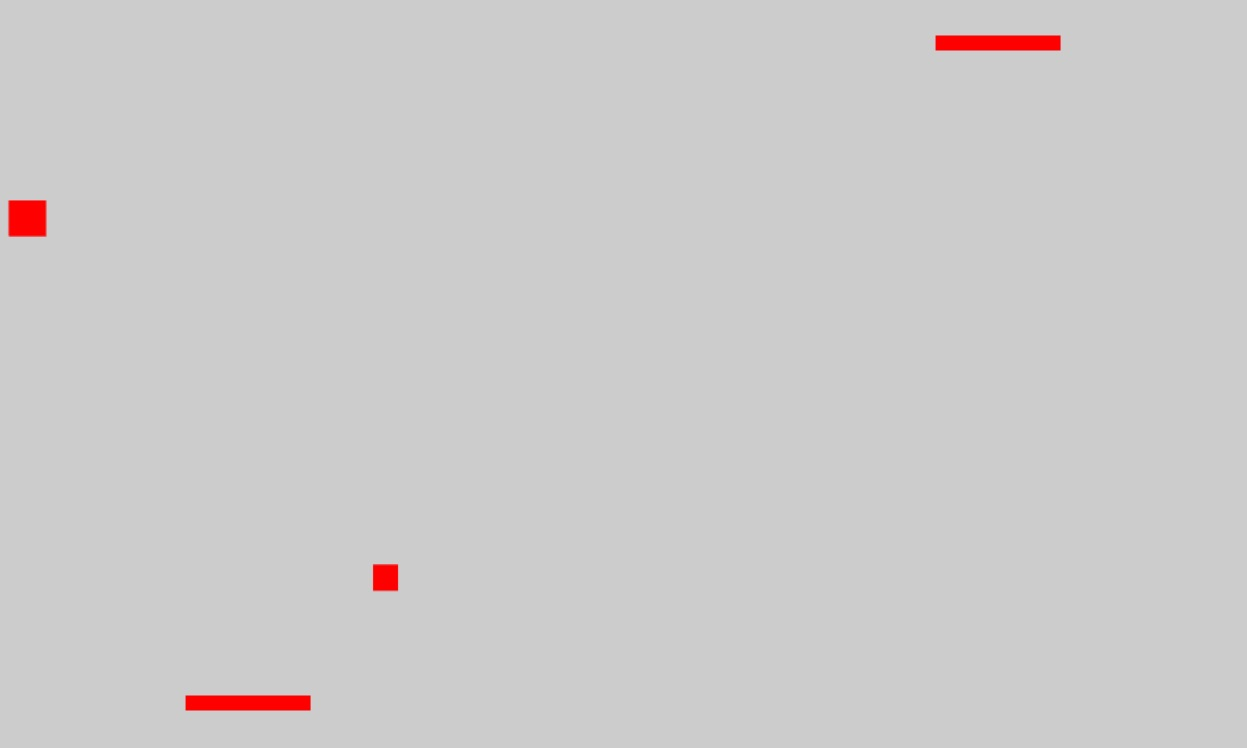
\includegraphics[scale=0.25]{3}
  	\caption{Mynd 1}
\end{figure}

Á myndum 2 og 3 má sjá að boltinn birtist á slembistað á bilinu $[-0.5,0.5]$ á lóðrétta ásnum og með slembistefnu. Forritinu er gefinn byrjunarhraði, svo er tölvan beðin um slembitölu á bilinu $[0,2\pi[$ og hraðinn í $x$ og $y$ stefnur er reiknaður út frá því með hornaföllum. Boltinn skoppar af hliðarveggjum og spöðum en getur farið út úr striganum uppi og niðri. Einnig eykst hraðinn á 2000 ramma fresti og gerir leikinn meira krefjandi.
\begin{figure}[h!]
	\centering
  	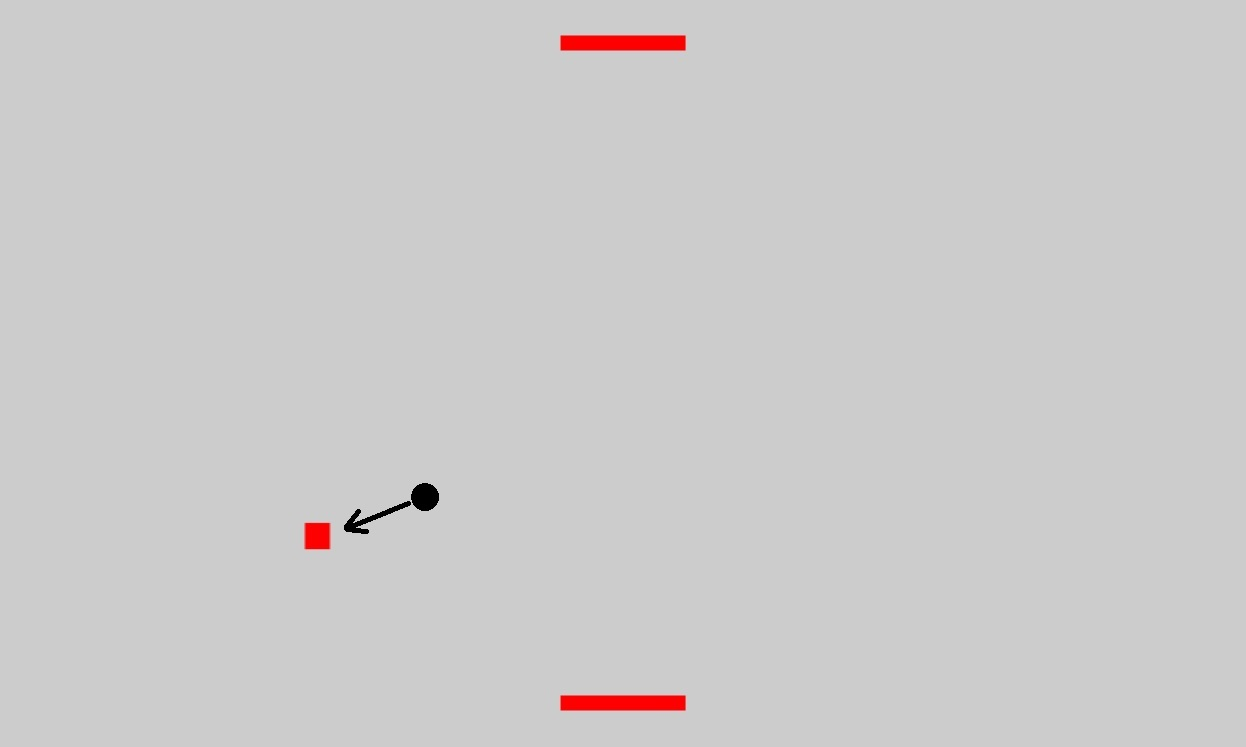
\includegraphics[scale=0.25]{1}
  	\caption{Mynd 2}
  	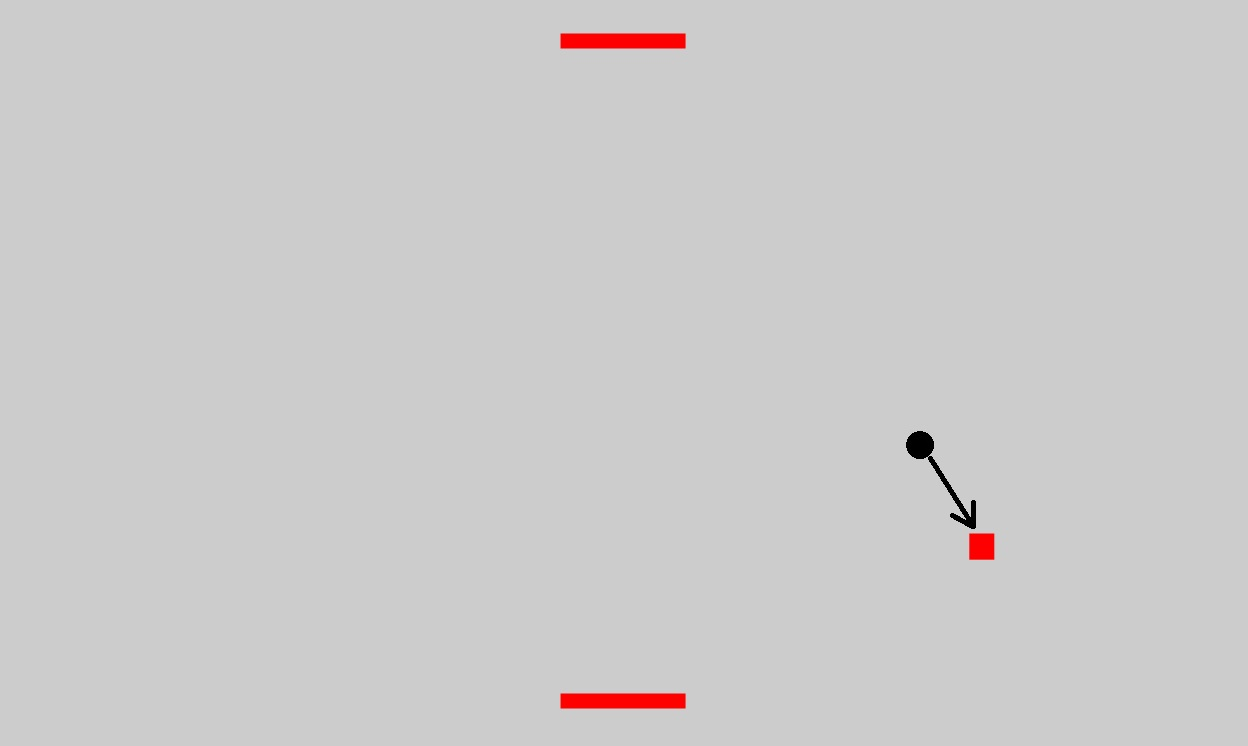
\includegraphics[scale=0.25]{2}
  	\caption{Mynd 3}
\end{figure}
\clearpage

Á 1000 ramma fresti birtist stig sem hægt er að ná og leikurinn telst unninn þegar að 10 stigum hefur verið náð. Ef að stig er nú þegar sýnilegt þegar að nýtt stig ætti að birtast, þá birtist það ekki. Stigið lýtur svipað út og boltinn en er ögn stærra. Á mynd 4 má sjá þegar boltinn er í þann mund að ná stigi.\\
\begin{figure}[h!]
	\centering
  	
\includegraphics[scale=0.25]{4}
  	\caption{Mynd 4}
\end{figure}\\
Undir striganum eru tveir skilaboðagluggar. Annar heldur utan um stigin sem þú hefur náð en hinn segir annað hvort "Leik lokið" $\text{}$ ef að boltinn fer út af striganum eða "Til hamingju, þú vannst!" $\text{}$ ef að leikmaður nær 10 stigum. Á mynd 5 má sjá dæmi um leik þar sem að spilari náði 5 stigum og misti svo boltann út fyrir gluggann.
\begin{figure}[h!]
	\centering
  	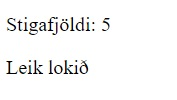
\includegraphics[scale=1]{5}
  	\caption{Mynd 5}
\end{figure}

Verkefnið má sjá í heild sinni á slóðinni:\\
\url{https://notendur.hi.is/~jgs7/tolvugrafik/Verkefni%201/v1.html}
\end{small}
\end{document}